\documentclass[,aspectratio=43]{beamer}

% ------------------------------------------------------------------------------
% Load theme -------------------------------------------------------------------
% ------------------------------------------------------------------------------
\usetheme[]{ubd}

% Information for the title page -----------------------------------------------
\author{Haziq Jamil}

\title{UBD Beamer Theme using RMarkdown}

\title{UBD Beamer Theme using RMarkdown}

\subtitle{An example presentation document with R code}

\institute{Mathematical Sciences, Faculty of Science, UBD\\
\url{https://haziqj.ml}}

\date{\today}

% ------------------------------------------------------------------------------
% knitr stuff ------------------------------------------------------------------
% ------------------------------------------------------------------------------
\usepackage{color}
\usepackage{fancyvrb}
\newcommand{\VerbBar}{|}
\newcommand{\VERB}{\Verb[commandchars=\\\{\}]}
\DefineVerbatimEnvironment{Highlighting}{Verbatim}{commandchars=\\\{\}}
% Add ',fontsize=\small' for more characters per line
\usepackage{framed}
\definecolor{shadecolor}{HTML}{F5F5F5}
\newenvironment{Shaded}{\begin{snugshade}}{\end{snugshade}}
\newcommand{\AlertTok}[1]{\textcolor[rgb]{0.94,0.16,0.16}{#1}}
\newcommand{\AnnotationTok}[1]{\textcolor[rgb]{0.56,0.35,0.01}{\textbf{\textit{#1}}}}
\newcommand{\AttributeTok}[1]{\textcolor[rgb]{0.77,0.63,0.00}{#1}}
\newcommand{\BaseNTok}[1]{\textcolor[rgb]{0.00,0.00,0.81}{#1}}
\newcommand{\BuiltInTok}[1]{#1}
\newcommand{\CharTok}[1]{\textcolor[rgb]{0.31,0.60,0.02}{#1}}
\newcommand{\CommentTok}[1]{\textcolor[rgb]{0.56,0.35,0.01}{\textit{#1}}}
\newcommand{\CommentVarTok}[1]{\textcolor[rgb]{0.56,0.35,0.01}{\textbf{\textit{#1}}}}
\newcommand{\ConstantTok}[1]{\textcolor[rgb]{0.00,0.00,0.00}{#1}}
\newcommand{\ControlFlowTok}[1]{\textcolor[rgb]{0.13,0.29,0.53}{\textbf{#1}}}
\newcommand{\DataTypeTok}[1]{\textcolor[rgb]{0.13,0.29,0.53}{#1}}
\newcommand{\DecValTok}[1]{\textcolor[rgb]{0.00,0.00,0.81}{#1}}
\newcommand{\DocumentationTok}[1]{\textcolor[rgb]{0.56,0.35,0.01}{\textbf{\textit{#1}}}}
\newcommand{\ErrorTok}[1]{\textcolor[rgb]{0.64,0.00,0.00}{\textbf{#1}}}
\newcommand{\ExtensionTok}[1]{#1}
\newcommand{\FloatTok}[1]{\textcolor[rgb]{0.00,0.00,0.81}{#1}}
\newcommand{\FunctionTok}[1]{\textcolor[rgb]{0.00,0.00,0.00}{#1}}
\newcommand{\ImportTok}[1]{#1}
\newcommand{\InformationTok}[1]{\textcolor[rgb]{0.56,0.35,0.01}{\textbf{\textit{#1}}}}
\newcommand{\KeywordTok}[1]{\textcolor[rgb]{0.13,0.29,0.53}{\textbf{#1}}}
\newcommand{\NormalTok}[1]{#1}
\newcommand{\OperatorTok}[1]{\textcolor[rgb]{0.81,0.36,0.00}{\textbf{#1}}}
\newcommand{\OtherTok}[1]{\textcolor[rgb]{0.56,0.35,0.01}{#1}}
\newcommand{\PreprocessorTok}[1]{\textcolor[rgb]{0.56,0.35,0.01}{\textit{#1}}}
\newcommand{\RegionMarkerTok}[1]{#1}
\newcommand{\SpecialCharTok}[1]{\textcolor[rgb]{0.00,0.00,0.00}{#1}}
\newcommand{\SpecialStringTok}[1]{\textcolor[rgb]{0.31,0.60,0.02}{#1}}
\newcommand{\StringTok}[1]{\textcolor[rgb]{0.31,0.60,0.02}{#1}}
\newcommand{\VariableTok}[1]{\textcolor[rgb]{0.00,0.00,0.00}{#1}}
\newcommand{\VerbatimStringTok}[1]{\textcolor[rgb]{0.31,0.60,0.02}{#1}}
\newcommand{\WarningTok}[1]{\textcolor[rgb]{0.56,0.35,0.01}{\textbf{\textit{#1}}}}
\usepackage{graphicx,grffile}
\makeatletter
\def\maxwidth{\ifdim\Gin@nat@width>\linewidth\linewidth\else\Gin@nat@width\fi}
\def\maxheight{\ifdim\Gin@nat@height>\textheight\textheight\else\Gin@nat@height\fi}
\makeatother
% Scale images if necessary, so that they will not overflow the page
% margins by default, and it is still possible to overwrite the defaults
% using explicit options in \includegraphics[width, height, ...]{}
\setkeys{Gin}{width=\maxwidth,height=\maxheight,keepaspectratio}
% Set default figure placement to htbp
\makeatletter
\def\fps@figure{htbp}
\makeatother
\setlength{\emergencystretch}{3em} % prevent overfull lines
\providecommand{\tightlist}{%
  \setlength{\itemsep}{0pt}\setlength{\parskip}{0pt}}
\setcounter{secnumdepth}{-\maxdimen} % remove section numbering

% ------------------------------------------------------------------------------
% Packages ---------------------------------------------------------------------
% ------------------------------------------------------------------------------

\usepackage{empheq}
\usepackage{ragged2e}
\usepackage{xltabular,longtable,booktabs,multirow,multicol,colortbl}

% \usepackage{caption}
% % Make caption package work with longtable
% \makeatletter
% \def\fnum@table{\tablename~\thetable}
% \makeatother

% highlight stuff using \hlc
\usepackage{soul}
\sethlcolor{ubdyellow}
\makeatletter
\let\HL\hl
\renewcommand\hl{%
  \let\set@color\beamerorig@set@color
  \let\reset@color\beamerorig@reset@color
  \HL}
\makeatother
% https://tex.stackexchange.com/questions/460731/highlight-color-a-part-of-text-in-block-in-beamer
\newcommand{\hlc}[2][ubdyellow]{{%
    \colorlet{foo}{#1}%
    \sethlcolor{foo}\hl{#2}}%
}
% https://tex.stackexchange.com/questions/352956/how-to-highlight-text-with-an-arbitrary-color

% To use arabic ----------------------------------------------------------------
% WARNING: Using arabic script causes some issues with footnotes.
% Packages are not loaded by default
\usepackage{polyglossia}  
\setdefaultlanguage{english}
\setotherlanguage{arabic} % to use arabic
\newfontfamily\arabicfontsf[Script=Arabic]{Amiri}
% Note that when arabic is set, the itemize becomes triangles
\setbeamertemplate{itemize item}[circ]
\setbeamertemplate{itemize subitem}[circ]
\setbeamertemplate{itemize subsubitem}[circ]
\usepackage{xeCJK}
\setCJKmainfont{SimSun}
\setCJKsansfont{FangSong}
\setCJKmonofont{KaiTi}

% % Fix for footnotes not showing when arabic script used
% % https://tex.stackexchange.com/questions/228075/beamer-in-arabic-language-doesnt-accept-footnotes
% \makeatletter
% \let\@footnotetext=\beamer@framefootnotetext
% \makeatother

% % Fix for footnotes not showing when using \footnote<.->
% \let\oldfootnote\footnote
% \renewcommand{\footnote}{\only<+->\oldfootnote}
% % https://stackoverflow.com/questions/62345074/show-footnote-only-after-a-pause-in-beamer-with-r-markdown

% Bibliography -----------------------------------------------------------------
\usepackage[style=authoryear,maxcitenames=2,maxbibnames=99,backend=biber,natbib]{biblatex}
\renewcommand*{\mkbibacro}[1]{#1}  % fix URL, DOI, ISBN, etc. font
\addbibresource{refs.bib}

% ------------------------------------------------------------------------------
% Mathematics ------------------------------------------------------------------
% ------------------------------------------------------------------------------

% coloured box around theorems etc.
\usepackage[skins,theorems]{tcolorbox}
\tcbset{highlight math style={enhanced,
  colframe=ubdblue,colback=white,arc=2pt,boxrule=1pt}}

\usepackage{amsmath,amssymb}
\usepackage{dsfont}  % for indicator variables \mathsds{1}
\usepackage{bm}  % for better bold script
\usepackage[makeroom]{cancel}
\usepackage{centernot}
\renewcommand{\CancelColor}{\color{gray}}
\newcommand{\bzero}{{\bm 0}}
\newcommand{\bone}{{\bm 1}}
\newcommand{\ba}{{\bm a}}
\newcommand{\bb}{{\bm b}}
\newcommand{\bc}{{\bm c}}
\newcommand{\bd}{{\bm d}}
\newcommand{\be}{{\bm e}}
\newcommand{\bff}{{\bm f}}
\newcommand{\bg}{{\bm g}}
\newcommand{\bh}{{\bm h}}
\newcommand{\bi}{{\bm i}}
\newcommand{\bj}{{\bm j}}
\newcommand{\bk}{{\bm k}}
\newcommand{\bl}{{\bm l}}
\newcommand{\bmm}{{\bm m}}
\newcommand{\bn}{{\bm n}}
\newcommand{\bo}{{\bm o}}
\newcommand{\bp}{{\bm p}}
\newcommand{\bq}{{\bm q}}
\newcommand{\br}{{\bm r}}
\newcommand{\bs}{{\bm s}}
\newcommand{\bt}{{\bm t}}
\newcommand{\bu}{{\bm u}}
\newcommand{\bv}{{\bm v}}
\newcommand{\bw}{{\bm w}}
\newcommand{\bx}{{\bm x}}
\newcommand{\by}{{\bm y}}
\newcommand{\bz}{{\bm z}}
\newcommand{\bA}{{\bm A}}
\newcommand{\bB}{{\bm B}}
\newcommand{\bC}{{\bm C}}
\newcommand{\bD}{{\bm D}}
\newcommand{\bE}{{\bm E}}
\newcommand{\bF}{{\bm F}}
\newcommand{\bG}{{\bm G}}
\newcommand{\bH}{{\bm H}}
\newcommand{\bI}{{\bm I}}
\newcommand{\bJ}{{\bm J}}
\newcommand{\bK}{{\bm K}}
\newcommand{\bL}{{\bm L}}
\newcommand{\bM}{{\bm M}}
\newcommand{\bN}{{\bm N}}
\newcommand{\bO}{{\bm O}}
\newcommand{\bP}{{\bm P}}
\newcommand{\bQ}{{\bm Q}}
\newcommand{\bR}{{\bm R}}
\newcommand{\bS}{{\bm S}}
\newcommand{\bT}{{\bm T}}
\newcommand{\bU}{{\bm U}}
\newcommand{\bV}{{\bm V}}
\newcommand{\bW}{{\bm W}}
\newcommand{\bX}{{\bm X}}
\newcommand{\bY}{{\bm Y}}
\newcommand{\bZ}{{\bm Z}}

% Greek bold letters
\newcommand{\balpha}{{\bm\alpha}}
\newcommand{\bbeta}{{\bm\beta}}
\newcommand{\bgamma}{{\bm\gamma}}
\newcommand{\bdelta}{{\bm\delta}}
\newcommand{\bepsilon}{{\bm\epsilon}}
\newcommand{\bvarepsilon}{{\bm\varepsilon}}
\newcommand{\bzeta}{{\bm\zeta}}
\newcommand{\bfeta}{{\bm\eta}}
\newcommand{\boldeta}{{\bm\eta}}
\newcommand{\btheta}{{\bm\theta}}
\newcommand{\bvartheta}{{\bm\vartheta}}
\newcommand{\biota}{{\bm\iota}}
\newcommand{\bkappa}{{\bm\kappa}}
\newcommand{\blambda}{{\bm\lambda}}
\newcommand{\bmu}{{\bm\mu}}
\newcommand{\bnu}{{\bm\nu}}
\newcommand{\bxi}{{\bm\xi}}
\newcommand{\bpi}{{\bm\pi}}
\newcommand{\bvarpi}{{\bm\varpi}}
\newcommand{\brho}{{\bm\rho}}
\newcommand{\bvarrho}{{\bm\varrho}}
\newcommand{\bsigma}{{\bm\sigma}}
\newcommand{\bvarsigma}{{\bm\varsigma}}
\newcommand{\btau}{{\bm\tau}}
\newcommand{\bupsilon}{{\bm\upsilon}}
\newcommand{\bphi}{{\bm\phi}}
\newcommand{\bvarphi}{{\bm\varphi}}
\newcommand{\bchi}{{\bm\chi}}
\newcommand{\bpsi}{{\bm\psi}}
\newcommand{\bomega}{{\bm\omega}}

\newcommand{\bGamma}{{\bm\Gamma}}
\newcommand{\bDelta}{{\bm\Delta}}
\newcommand{\bTheta}{{\bm\Theta}}
\newcommand{\bLambda}{{\bm\Lambda}}
\newcommand{\bXi}{{\bm\Xi}}
\newcommand{\bPi}{{\bm\Pi}}
\newcommand{\bSigma}{{\bm\Sigma}}
\newcommand{\bUpsilon}{{\bm\Upsilon}}
\newcommand{\bPhi}{{\bm\Phi}}
\newcommand{\bPsi}{{\bm\Psi}}
\newcommand{\bOmega}{{\bm\Omega}}

% Probability and Statistics
\DeclareMathOperator{\Prob}{P}
\DeclareMathOperator{\E}{E}
\DeclareMathOperator{\Var}{Var}
\DeclareMathOperator{\Cov}{Cov}
\DeclareMathOperator{\Corr}{Corr}
\DeclareMathOperator{\sd}{sd}
\DeclareMathOperator{\se}{se}
\DeclareMathOperator{\N}{N}
\DeclareMathOperator{\Bin}{Bin}
\DeclareMathOperator{\Bern}{Bern}
\DeclareMathOperator{\Dir}{Dir}
\DeclareMathOperator{\Wis}{Wis}
\DeclareMathOperator{\logit}{logit}
\DeclareMathOperator{\expit}{expit}
\DeclareMathOperator{\Mult}{Mult}
\DeclareMathOperator{\Cat}{Cat}
\DeclareMathOperator{\Pois}{Poi}
\DeclareMathOperator{\Geom}{Geom}
\DeclareMathOperator{\NBin}{NBin}
\DeclareMathOperator{\Exp}{Exp}
\DeclareMathOperator{\Betadist}{Beta}
\DeclareMathOperator{\Hypergeom}{Hypergeom}
\DeclareMathOperator{\Cauchy}{Cauchy}
\DeclareMathOperator{\hCauchy}{half-Cauchy}
\DeclareMathOperator{\LKJ}{LKJ}
\DeclareMathOperator{\Unif}{Unif}
\DeclareMathOperator{\KL}{KL}
\DeclareMathOperator{\ind}{\mathds{1}}
\newcommand{\iid}{\,\overset{\text{iid}}{\sim}\,}
\DeclareMathOperator*{\plim}{plim}
\DeclareMathOperator{\Lik}{L}
\DeclareMathOperator{\Leb}{Leb}

% Blackboard bold
\newcommand{\bbR}{\mathbb{R}}
\newcommand{\bbN}{\mathbb{N}}
\newcommand{\bbZ}{\mathbb{Z}}
\newcommand{\bbC}{\mathbb{C}}
\newcommand{\bbS}{\mathbb{S}}
\newcommand{\bbH}{\mathbb{H}}
\newcommand{\bbP}{\mathbb{P}}
\newcommand{\bbQ}{\mathbb{Q}}
\newcommand{\bbE}{\mathbb{E}}

% Math calligraphic fonts
\newcommand{\cA}{{\mathcal A}}
\newcommand{\cB}{{\mathcal B}}
\newcommand{\cC}{{\mathcal C}}
\newcommand{\cD}{{\mathcal D}}
\newcommand{\cE}{{\mathcal E}}
\newcommand{\cF}{{\mathcal F}}
\newcommand{\cG}{{\mathcal G}}
\newcommand{\cH}{{\mathcal H}}
\newcommand{\cI}{{\mathcal I}}
\newcommand{\cJ}{{\mathcal J}}
\newcommand{\cK}{{\mathcal K}}
\newcommand{\cL}{{\mathcal L}}
\newcommand{\cM}{{\mathcal M}}
\newcommand{\cN}{{\mathcal N}}
\newcommand{\cO}{{\mathcal O}}
\newcommand{\cP}{{\mathcal P}}
\newcommand{\cQ}{{\mathcal Q}}
\newcommand{\cR}{{\mathcal R}}
\newcommand{\cS}{{\mathcal S}}
\newcommand{\cT}{{\mathcal T}}
\newcommand{\cU}{{\mathcal U}}
\newcommand{\cV}{{\mathcal V}}
\newcommand{\cW}{{\mathcal W}}
\newcommand{\cX}{{\mathcal X}}
\newcommand{\cY}{{\mathcal Y}}
\newcommand{\cZ}{{\mathcal Z}}

% Overbrace and underbrace
\newcommand{\myoverbrace}[3][gray!70]{{\color{#1}\overbrace{\color{black}#2}^{#3}}}
\newcommand{\myunderbrace}[3][gray!70]{{\color{#1}\underbrace{\color{black}#2}_{#3}}}

% Conveniences
\newcommand{\const}{\text{const.}}
\newcommand{\half}[1][1]{\frac{#1}{2}}  % \half for 1/2 or \half[n] for n/2, etc.
\DeclareMathOperator{\diag}{diag}
\DeclareMathOperator{\tr}{tr}
\DeclareMathOperator*{\argmin}{arg\,min}
\DeclareMathOperator*{\argmax}{arg\,max}

% Comments gray text
\newcommand{\mycomment}[2][10pt]{\hspace{#1}\rlap{\color{gray}\text{#2}}}

% Derivatives and integration
\let\d\relax
\DeclareMathOperator{\dd}{d}
\newcommand{\dint}{\dd\hspace{0.5pt}\!}
\newcommand{\d}{\text{d}}

% https://tex.stackexchange.com/questions/19981/how-to-write-rudins-symbol-for-absolute-continuity-of-measures
\DeclareFontFamily{U}{matha}{\hyphenchar\font45}
\DeclareFontShape{U}{matha}{m}{n}{
  <-6> matha5 <6-7> matha6 <7-8> matha7
  <8-9> matha8 <9-10> matha9
  <10-12> matha10 <12-> matha12
  }{}
\DeclareSymbolFont{matha}{U}{matha}{m}{n}
\DeclareMathSymbol{\Lt}{3}{matha}{"CE}

\usepackage{lipsum}
\SetLipsumLanguage{english}

\graphicspath{ {figure/} }

\begin{document}

\begin{frame}[plain,noframenumbering]
	\titlepage
\end{frame}

\begin{frame}[plain,noframenumbering]{Overview}
    \tableofcontents
  \end{frame}

\hypertarget{introduction}{%
\section{Introduction}\label{introduction}}

\begin{frame}{Introduction}
The UBD Beamer Theme is a modern and minimal theme designed for getting
information across in a clean and uncluttered manner. \bigskip

This theme is based on the
\href{https://github.com/kailashbuki/beamerthemesaarland}{Saarland
Beamer Theme}, with its logos and fonts changed, and colour scheme
adapted to UBD's official brand colours.
\end{frame}

\hypertarget{features}{%
\section{Features}\label{features}}

\hypertarget{lists}{%
\subsection{Lists}\label{lists}}

\begin{frame}{Slide full of lists}
\protect\hypertarget{slide-full-of-lists}{}
\emph{Universiti Brunei Darussalam} (UBD; translation University of
Brunei Darussalam; Jawi: \textarabic{يونيبرسيتي بروني دارالسلام}) is the
first university in Brunei.

\begin{itemize}
\tightlist
\item
  UBD in figures

  \begin{itemize}
  \tightlist
  \item
    \textbf{Established}: 1985
  \item
    \textbf{Medium of instruction}: English
  \item
    \textbf{Academic faculties}: 9
  \item
    \textbf{Research Institutes}: 7
  \item
    \textbf{Student enrolment}: 3,137 (in 2015, approx.)
  \end{itemize}
\item
  History

  \begin{itemize}
  \tightlist
  \item
    \textbf{1985}: UBD established, first campus in Gadong
  \item
    \textbf{1995}: UBD moved to Tungku Link
  \item
    \textbf{2009}: Introduction of
    \href{https://ubd.edu.bn/admission/undergraduate/gennext-degree-programme/}{GenNEXT
    Programme}
  \item
    \textbf{2011}: Commencement of the first Discovery Year programme\\
  \end{itemize}
\item
  Credits: \url{https://ubd.edu.bn/} and Wikipedia
\end{itemize}
\end{frame}

\hypertarget{blocks}{%
\subsection{Blocks}\label{blocks}}

\begin{frame}[fragile]{Blocks}
\begin{block}{Standard Block}
\protect\hypertarget{standard-block}{}
This is a standard block using the \texttt{block} environment.
\end{block}

\begin{exampleblock}{Example Block}
This is an example block using the \texttt{exampleblock} environment.

\end{exampleblock}

\begin{alertblock}{Alert Block}
This is an alert block using the \texttt{alertblock} environment.

\end{alertblock}

\begin{altblock}{Alternative Block}
This is an alternatively-coloured block using the \texttt{altblock}
environment.

\end{altblock}
\end{frame}

\hypertarget{quotes}{%
\subsection{Quotes}\label{quotes}}

\begin{frame}{Quotation}
\protect\hypertarget{quotation}{}
\begin{quote}
Archimedes will be remembered when Aeschylus is forgotten, because
languages die and mathematical ideas do not. ``Immortality'' may be a
silly word, but probably a mathematician has the best chance of whatever
it may mean.
\end{quote}

\hfill --- G. H. Hardy in \emph{A Mathematician's Apology, 1941}
\end{frame}

\hypertarget{columns}{%
\subsection{Columns}\label{columns}}

\begin{frame}{Two columns}
\protect\hypertarget{two-columns}{}
We can also add two columns in the slides.\bigskip

\begin{columns}[T]
\begin{column}{0.48\textwidth}
This is the first column. In this column, we can also add a block for
instance.

\begin{block}{Block}
\protect\hypertarget{block}{}
I am a block in a column.
\end{block}
\end{column}

\begin{column}{0.48\textwidth}
\begin{itemize}
\tightlist
\item
  In this column,
\item
  we just add the
\item
  bullet points.
\end{itemize}
\end{column}
\end{columns}
\end{frame}

\hypertarget{colour-palette}{%
\subsection{Colour palette}\label{colour-palette}}

\begin{frame}[fragile]{Colour palette}
\begin{itemize}
\tightlist
\item
  \textcolor{ubdblue}{Blues: \texttt{ubdblue} a.k.a. Y In Mn Blue
  (\#325494)}
\item
  \textcolor{ubdteal}{Teals: \texttt{ubdteal} a.k.a. Medium Aquamarine
  (\#58DDB3)}
\item
  \textcolor{ubdyellow}{Yellows: \texttt{ubdyellow} a.k.a. Maize Crayola
  Red (\#F5C946)}
\item
  \textcolor{ubdred}{Alerted text: \texttt{ubdred} a.k.a. Upsdell Red
  (\#B10F2E)}
\item
  \textcolor{ubdblack}{Normal text: \texttt{ubdblack} a.k.a. Dark Sienna
  (\#230C0F)}
\item
  \textcolor{gray}{Grays: \texttt{gray} a.k.a. Spanish Gray (\#999999)}
\end{itemize}

\blfootnote{\url{https://coolors.co/palette/325494-58ddb3-f5c946-b10f2e-230c0f}}
\end{frame}

\begin{frame}[fragile]{Fonts}
\protect\hypertarget{fonts}{}
The font is left to the default beamer font (which I believe is the
Computer Modern). In order to get the sans-serif fonts for the
mathematics (including the greek letters), the following lines are
called in the \texttt{.sty} file:

\begin{Shaded}
\begin{Highlighting}[]
\BuiltInTok{\textbackslash{}usepackage}\NormalTok{\{}\ExtensionTok{cmbright}\NormalTok{\}}
\FunctionTok{\textbackslash{}usefonttheme}\NormalTok{\{professionalfonts\}}
\end{Highlighting}
\end{Shaded}

So compiling using pdf\LaTeX~should get the desired output. \medskip

On the other hand, compiling with Xe\LaTeX~seems to mess up the fonts,
probably because legacy fonts are loaded. There is a switch in the
\texttt{.sty} file which loads \texttt{fontspec} package to fix this
(kind of?).
\end{frame}

\hypertarget{mathematics}{%
\subsection{Mathematics}\label{mathematics}}

\begin{frame}{Mathematics}
Let \(X\) be a simple random variable defined on
\((\Omega,\mathcal F,\mathbb P)\) that takes on finitely many values
\(\{x_1,\dots,x_n\}\). The expectation of \(X\),
\(\operatorname{E}(X)\), is the Lebesgue integral of \(X\) with respect
to \(\mathbb P\), \[
\operatorname{E}(X) := \int X(\omega) \operatorname{d \mathbb P} = \sum_{i=1}^n x_i \operatorname{\mathbb P}(\omega \in A_i),
\] where \(A_i=\{\omega\in\Omega \mid X(\omega)=x_i \}\).

\vspace{-0.5em}

\begin{gather*}
AaBbCcDdEeFfGgHhIiJjKkLlMmNnOoPpQqRrSsTtUuVv\\WwXxYyZz \\[0.5em]
1234567890 \\[0.5em]
\alpha
 \beta
\Gamma  \gamma
\Delta  \delta
\epsilon  \varepsilon   
\zeta
\eta
\Theta \theta  \vartheta
\iota
\kappa  \varkappa
\Lambda  \lambda
\mu
\nu
\Xi  \xi
\Pi \pi  \varpi
\rho  
\Sigma \sigma 
\tau
\Upsilon  \upsilon
\Phi \phi  \varphi
\chi
\Psi  \psi
\Omega  \omega \\[0.5em]
\prod \oint \bigoplus \bigotimes \bigcup \bigcap 
\end{gather*}
\end{frame}

\begin{frame}{Theorems et al.}
\protect\hypertarget{theorems-et-al.}{}
\begin{definition}[Prime numbers]
A prime number is a natural number greater than 1 that is not a product
of two smaller natural numbers.
\end{definition}

\begin{theorem}[Infinitude of primes]
There are an infinite number of prime numbers.
\end{theorem}

\begin{proof}
Suppose that there exist only a finite number of primes,
\(p_1,\dots,p_n\), say. The number \[
N = 1+p_1\cdots p_n
\] is divisible by some prime \(p\). But \(p\) cannot be any of
\(p_1,\dots,p_n\), since the latter all leave remainder 1 on dividing
\(N\). This contradicts our assumption that \(p_1,\dots,p_n\) is the
complete list of primes.
\end{proof}
\end{frame}

\begin{frame}[fragile]{Example blocks}
\protect\hypertarget{example-blocks}{}
Example blocks are continuously numbered (using the \texttt{example}
environment).

\begin{example}[Examples of prime numbers]
The numbers

\begin{itemize}
\tightlist
\item
  2;
\item
  3;
\item
  5; and
\item
  7
\end{itemize}

are examples of prime numbers.
\end{example}

\begin{example}[Examples of non-prime numbers]
Since \(4 = 2 \times 2\), it is not a prime.
\end{example}
\end{frame}

\hypertarget{citations}{%
\subsection{Citations}\label{citations}}

\begin{frame}{Citations}
The importance of grounding one's self in elementary probability theory
and mathematical statistics cannot be overstated. Here are some
excellent fundamental textbooks every student of statistics should read:
\textcite{casella2002statistical}, \textcite{pawitan2001all}, and
\textcite{wasserman2013all}.

\blfootnote{It is highly suggested to use pandoc's way of generating bibliographies (see \href{https://rmarkdown.rstudio.com/authoring_bibliographies_and_citations.html}{here}) rather than using Biblatex. This footnote was created using the custom \texttt{\textbackslash blfootnote\{\}} command.}
\end{frame}

\hypertarget{using-r}{%
\subsection{\texorpdfstring{Using \texttt{R}}{Using R}}\label{using-r}}

\begin{frame}[fragile]{Syntax highlighting}
\protect\hypertarget{syntax-highlighting}{}
\begin{Shaded}
\begin{Highlighting}[]
\NormalTok{f }\OtherTok{\textless{}{-}} \ControlFlowTok{function}\NormalTok{(x) \{}
  \CommentTok{\# Check small prime}
  \ControlFlowTok{if}\NormalTok{ (x }\SpecialCharTok{\textgreater{}} \DecValTok{10} \SpecialCharTok{||}\NormalTok{ x }\SpecialCharTok{\textless{}} \SpecialCharTok{{-}}\DecValTok{10}\NormalTok{) \{}
    \FunctionTok{stop}\NormalTok{(}\StringTok{"Input too big"}\NormalTok{)}
\NormalTok{  \} }\ControlFlowTok{else} \ControlFlowTok{if}\NormalTok{ (x }\SpecialCharTok{\%in\%} \FunctionTok{c}\NormalTok{(}\DecValTok{2}\NormalTok{, }\DecValTok{3}\NormalTok{, }\DecValTok{5}\NormalTok{, }\DecValTok{7}\NormalTok{)) \{}
    \FunctionTok{cat}\NormalTok{(}\StringTok{"Input is prime!}\SpecialCharTok{\textbackslash{}n}\StringTok{"}\NormalTok{)}
\NormalTok{  \} }\ControlFlowTok{else} \ControlFlowTok{if}\NormalTok{ (x }\SpecialCharTok{\%\%} \DecValTok{2} \SpecialCharTok{==} \DecValTok{0}\NormalTok{) \{}
    \FunctionTok{cat}\NormalTok{(}\StringTok{"Input is even!}\SpecialCharTok{\textbackslash{}n}\StringTok{"}\NormalTok{)}
\NormalTok{  \} }\ControlFlowTok{else} \ControlFlowTok{if}\NormalTok{ (x }\SpecialCharTok{\%\%} \DecValTok{2} \SpecialCharTok{==} \DecValTok{1}\NormalTok{) \{}
    \FunctionTok{cat}\NormalTok{(}\StringTok{"Input is odd!}\SpecialCharTok{\textbackslash{}n}\StringTok{"}\NormalTok{)}
\NormalTok{  \}}
\NormalTok{\}}
\end{Highlighting}
\end{Shaded}
\end{frame}

\begin{frame}[fragile]{Slide with R Output}
\protect\hypertarget{slide-with-r-output}{}
\begin{Shaded}
\begin{Highlighting}[]
\FunctionTok{summary}\NormalTok{(cars)}
\end{Highlighting}
\end{Shaded}

\begin{verbatim}
##      speed           dist       
##  Min.   : 4.0   Min.   :  2.00  
##  1st Qu.:12.0   1st Qu.: 26.00  
##  Median :15.0   Median : 36.00  
##  Mean   :15.4   Mean   : 42.98  
##  3rd Qu.:19.0   3rd Qu.: 56.00  
##  Max.   :25.0   Max.   :120.00
\end{verbatim}
\end{frame}

\begin{frame}[fragile]{Slide with Plot}
\protect\hypertarget{slide-with-plot}{}
\vspace{-1em}

\begin{Shaded}
\begin{Highlighting}[]
\FunctionTok{ggplot}\NormalTok{(}\FunctionTok{tibble}\NormalTok{(}\AttributeTok{x =} \FunctionTok{rnorm}\NormalTok{(}\DecValTok{100}\NormalTok{), }\AttributeTok{y =} \FunctionTok{rnorm}\NormalTok{(}\DecValTok{100}\NormalTok{)), }\FunctionTok{aes}\NormalTok{(x, y)) }\SpecialCharTok{+}
  \FunctionTok{geom\_point}\NormalTok{()}
\end{Highlighting}
\end{Shaded}

\begin{center}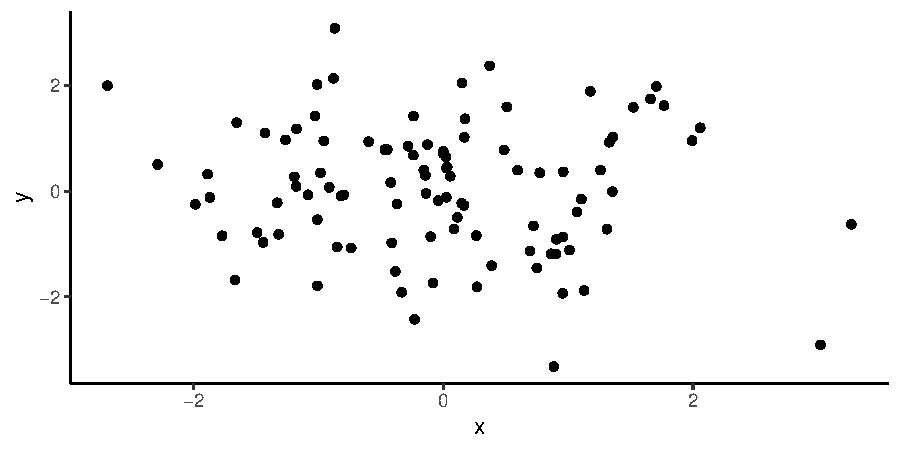
\includegraphics{figure/slideplot-1} \end{center}
\end{frame}

\hypertarget{conclusion}{%
\section{Conclusion}\label{conclusion}}

\begin{frame}[fragile]{Conclusion}
To use this theme, download and place the following files and folders
into your working directory:

\begin{enumerate}
\tightlist
\item
  \texttt{beamerthemeUBD.sty} (the beamer theme)
\item
  \texttt{ubd\_beamer\_rmd.tex} (the Rmd beamer template)
\item
  \texttt{luafilters/} (the lua filters in the folder)
\item
  \texttt{ubd\_brand.pdf} (the university logo)
\end{enumerate}

To start, you may use the \texttt{slides\_rmd.Rmd} as a guide and edit
from there.

\begin{block}{For non-Rmd beamer}
\protect\hypertarget{for-non-rmd-beamer}{}
All you need is 1. and 4. (the Rmd template and lua filters are not
necessary). See the file \texttt{minimal\_example.tex}.
\end{block}
\end{frame}

\begin{frame}[plain,noframenumbering]{End}
\protect\hypertarget{end}{}
\centering
\Huge

\textcolor{ubdblue}{Thank you!}
\end{frame}

\begin{frame}[t,allowframebreaks,noframenumbering,plain]{References}
\protect\hypertarget{references}{}
\printbibliography[heading=none]

\appendix
\backupbegin
\end{frame}

\hypertarget{backup-slides}{%
\section{Backup slides}\label{backup-slides}}

\begin{frame}[fragile]{Backup slides}
Often times in a presentation, we don't have enough time to present
everything, but it's a good idea to prepare backup slides in case the
audience asks about it afterwards.\bigskip

We can achieve that using the \texttt{\textbackslash{}appendix} usage.
\end{frame}

\hypertarget{backup-topic-1}{%
\section{Backup topic 1}\label{backup-topic-1}}

\begin{frame}{Backup topic 1}
\lipsum[1]
\end{frame}

\hypertarget{backup-topic-2}{%
\section{Backup topic 2}\label{backup-topic-2}}

\begin{frame}{Backup topic 2}
\begin{block}{A block}
\protect\hypertarget{a-block}{}
\lipsum[4]
\end{block}
\end{frame}



\backupend

\end{document}		